% Title: gl2ps_renderer figure
% Creator: GL2PS 1.4.0, (C) 1999-2017 C. Geuzaine
% For: Octave
% CreationDate: Fri Jul 09 00:00:52 2021
\setlength{\unitlength}{1pt}
\begin{picture}(0,0)
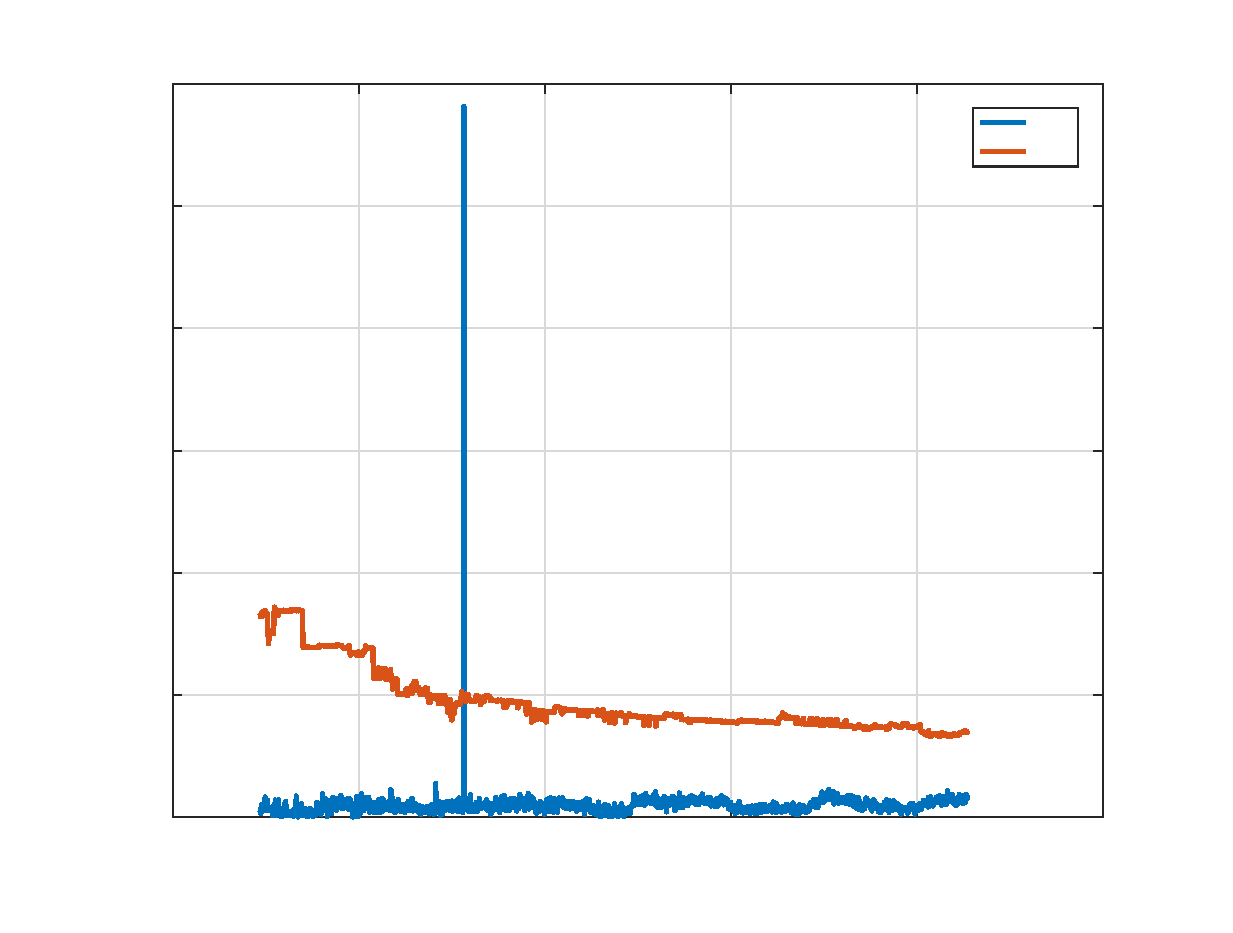
\includegraphics{images\p3\HPE_HPL-inc}
\end{picture}%
\begin{picture}(576,432)(0,0)
\fontsize{10}{0}
\selectfont\put(74.88,40.0183){\makebox(0,0)[t]{\textcolor[rgb]{0.15,0.15,0.15}{{115000}}}}
\fontsize{10}{0}
\selectfont\put(164.159,40.0183){\makebox(0,0)[t]{\textcolor[rgb]{0.15,0.15,0.15}{{116000}}}}
\fontsize{10}{0}
\selectfont\put(253.44,40.0183){\makebox(0,0)[t]{\textcolor[rgb]{0.15,0.15,0.15}{{117000}}}}
\fontsize{10}{0}
\selectfont\put(342.719,40.0183){\makebox(0,0)[t]{\textcolor[rgb]{0.15,0.15,0.15}{{118000}}}}
\fontsize{10}{0}
\selectfont\put(432,40.0183){\makebox(0,0)[t]{\textcolor[rgb]{0.15,0.15,0.15}{{119000}}}}
\fontsize{10}{0}
\selectfont\put(521.28,40.0183){\makebox(0,0)[t]{\textcolor[rgb]{0.15,0.15,0.15}{{120000}}}}
\fontsize{10}{0}
\selectfont\put(69.8752,47.52){\makebox(0,0)[r]{\textcolor[rgb]{0.15,0.15,0.15}{{0}}}}
\fontsize{10}{0}
\selectfont\put(69.8752,106.2){\makebox(0,0)[r]{\textcolor[rgb]{0.15,0.15,0.15}{{10}}}}
\fontsize{10}{0}
\selectfont\put(69.8752,164.88){\makebox(0,0)[r]{\textcolor[rgb]{0.15,0.15,0.15}{{20}}}}
\fontsize{10}{0}
\selectfont\put(69.8752,223.56){\makebox(0,0)[r]{\textcolor[rgb]{0.15,0.15,0.15}{{30}}}}
\fontsize{10}{0}
\selectfont\put(69.8752,282.24){\makebox(0,0)[r]{\textcolor[rgb]{0.15,0.15,0.15}{{40}}}}
\fontsize{10}{0}
\selectfont\put(69.8752,340.92){\makebox(0,0)[r]{\textcolor[rgb]{0.15,0.15,0.15}{{50}}}}
\fontsize{10}{0}
\selectfont\put(69.8752,399.6){\makebox(0,0)[r]{\textcolor[rgb]{0.15,0.15,0.15}{{60}}}}
\fontsize{11}{0}
\selectfont\put(298.08,27.0183){\makebox(0,0)[t]{\textcolor[rgb]{0.15,0.15,0.15}{{Tempo (s)}}}}
\fontsize{11}{0}
\selectfont\put(52.8754,223.56){\rotatebox{90}{\makebox(0,0)[b]{\textcolor[rgb]{0.15,0.15,0.15}{{HPE e HPL (m)}}}}}
\fontsize{9}{0}
\selectfont\put(487.768,380.971){\makebox(0,0)[l]{\textcolor[rgb]{0,0,0}{{HPE}}}}
\fontsize{9}{0}
\selectfont\put(487.768,366.937){\makebox(0,0)[l]{\textcolor[rgb]{0,0,0}{{HPL}}}}
\end{picture}
